\chapter{Introduction}
\label{ch:introduction}

\setcounter{page}{1}
\pagenumbering{arabic}

\section{Networks everywhere}

Look closely at almost any complex system and you will find, hiding inside 
it, a network. A network, in the sense used throughout this book, is nothing 
more exotic than a collection of things together with a record of which pairs 
of them are connected. The ``things'' are drawn as dots and called 
\emph{nodes}. A connection between two of them is drawn as a line and called 
a \emph{link}. That is the whole vocabulary needed to begin: a network is 
dots and lines, nodes and links.

What is remarkable is how many different systems fit this simple picture. The 
Internet is a network whose nodes are routers and whose links are the cables 
between them. The World Wide Web is a network of pages connected by the 
hyperlinks you click. A society is a network of people connected by 
acquaintance, friendship, collaboration, or contact. A living cell contains a 
network of proteins connected when two of them physically interact, and 
another of chemicals connected by the reactions that turn one into another. A 
project is decomposed into discrete activities and the logical dependencies 
between them. The scientific literature is a network of papers connected by 
citations, and of authors connected when they write a paper together 
\citep{newman2001,newman2003,albert2002,dorogovtsev2002}. These systems share 
almost nothing on the surface --- one is silicon and glass, another is flesh 
and acquaintance, another is ink and ideas --- and yet, viewed as networks, 
they turn out to look astonishingly alike.

That likeness is the subject of this book. Over the past few decades, as
researchers gathered maps of real networks ranging from a handful of nodes to
billions, the same handful of features kept reappearing, no matter the system.
Four of them organize everything that follows, so it is worth meeting them in
plain language before we make them precise.

The first is the \emph{small-world} property \citep{watts1998}. In a real
network you can usually get from any node to any other in only a few hops, even
when the network is enormous --- the famous ``six degrees of separation'' between
any two people on Earth is one example. At the same time these networks are
highly \emph{cliquish}: your friends tend to be friends of one another, far more
than chance would predict. Short hops everywhere, plus dense little
neighborhoods: that combination is the small world.

The second is the \emph{scale-free} property \citep{barabasi1999,faloutsos1999}.
If you count how many connections each node has, you find that most nodes have
very few, while a small number --- the \emph{hubs} --- have a huge number.
Hollywood has a few actors who have worked with almost everyone and a multitude
who have appeared in one film; the Web has a few pages everybody links to and
billions that are barely linked at all. There is no ``typical'' number of
connections in such a network, which is what the term \emph{scale-free} is
meant to capture.

The third, more subtle and the real connective tissue of this book, is that real
networks carry systematic \emph{correlations} and a \emph{hierarchy}
\citep{pastorsatorras2001,vazquez2002,ravasz2003,vazquez2025}. Whom a node
connects to is not random with respect to how connected those neighbors are, and
the cliquishness around a node depends in a regular way on how many connections
the node has. We will make both of these ideas concrete in a moment.

The fourth, more recent and pitched at a larger scale than the rest, is that real
networks divide into \emph{communities}: groups of nodes densely connected among
themselves but only loosely tied to the rest. People cluster into social circles,
web pages into topics, proteins into functional modules --- so that a network
often looks less like one seamless fabric than a patchwork of tight-knit groups
stitched loosely together. Detecting these communities, and explaining why they
arise, has grown into a research field of its own
\citep{girvan2002,fortunato2010,palla2005}.

The central question of the book is not \emph{whether} these patterns exist ---
the evidence is by now overwhelming --- but \emph{where they come from}. The
answer we will develop, over and over in different settings, is that they need
not be designed in. They appear all by themselves in networks that grow
according to \emph{local rules}: rules in which each newly arriving node decides
where to attach using only what is right in front of it --- a node it has already
reached, and that node's immediate neighbors. No node ever needs to survey the
whole network. That a global pattern can emerge from purely local decisions is,
in one sentence, the thesis of this book.

\section{Some basic measures}

To talk about networks precisely we need a few simple measures. None of them is
harder than counting; we introduce them gently here and will lean on them in
every chapter. Throughout, we picture a network with $n$ nodes. When it helps to
be formal we use the \emph{adjacency matrix} $a_{ij}$, a bookkeeping device that
is simply $1$ if nodes $i$ and $j$ are connected and $0$ if they are not --- a
giant table of yes/no answers to ``are these two linked?''

\paragraph{Degree and degree distribution.}
The \emph{degree} of a node is its number of links --- how many neighbors it has.
We write it $k$, so a node with $k=3$ has three connections. (In formulas, the
degree of node $i$ is $k_i = \sum_j a_{ij}$, which just says: add up the
yes-answers in row $i$ of the table.) The \emph{degree distribution} $p(k)$ is
the recipe for how degrees are spread across the network: it is the fraction of
nodes that have exactly $k$ links, equivalently the chance that a node picked at
random has degree $k$.

A network is called \emph{scale-free} when this distribution follows a
\emph{power law},
\begin{equation}
  p(k) \sim k^{-\gamma},
  \label{eq:intro-powerlaw}
\end{equation}
where the symbol $\sim$ means ``behaves like'' for large $k$, and $\gamma$
(gamma) is a number, the \emph{exponent}, typically between $2$ and $3$ for real
networks. A power law is just a rule that says ``ten times bigger is some fixed
number of times rarer.'' Unlike the bell-shaped curves of everyday statistics
--- human heights, say, which cluster tightly around an average --- a power law
has a long, heavy tail: extremely well-connected hubs are rare but nowhere near
as rare as a bell curve would allow. This is why scale-free networks are
hub-dominated, and why those hubs end up running much of the show
(Figure~\ref{fig:intro-degree}).

\begin{figure}[t]
\centering
\begin{adjustbox}{max width=\linewidth}\begin{tikzpicture}[
  sm/.style={circle,draw=black!60,fill=black!5,minimum size=4mm,inner sep=0pt},
  md/.style={circle,draw=black!60,fill=black!8,minimum size=6mm,inner sep=0pt},
  hub/.style={circle,draw=accent!80!black,fill=black!30,minimum size=10mm,inner sep=0pt},
  lnk/.style={draw=black!40,line width=0.7pt}]
  \node[hub] (H) at (1.7,0.6) {};
  \node[sm] (n1) at (0.1,1.5)  {};
  \node[sm] (n2) at (-0.2,0.3) {};
  \node[sm] (n3) at (0.7,-0.8) {};
  \node[sm] (n4) at (2.0,1.9)  {};
  \node[sm] (n5) at (3.1,1.2)  {};
  \node[md] (n6) at (3.3,-0.3) {};
  \node[sm] (n7) at (2.1,-0.9) {};
  \node[sm] (m)  at (4.6,0.4)  {};
  \draw[lnk] (H)--(n1) (H)--(n2) (H)--(n3) (H)--(n4) (H)--(n5) (H)--(n6) (H)--(n7);
  \draw[lnk] (n6)--(m) (n5)--(m);
  \node[accent,font=\scriptsize] at (1.7,-0.45) {hub, $k=7$};
  \node[font=\scriptsize] at (4.6,-0.25) {$k=2$};
\end{tikzpicture}\end{adjustbox}
\caption{\textbf{Degree.} A node's degree is simply its number of links. Drawn
here with node size growing with degree: a few hubs (such as the central one,
$k=7$) carry many links, while most nodes have only one or two. That imbalance ---
many small nodes, a few giant hubs --- is the hallmark of a scale-free
network.}
\label{fig:intro-degree}
\end{figure}

\paragraph{Clustering coefficient.}
The \emph{clustering coefficient} measures cliquishness: of all the pairs of your
neighbors, what fraction are themselves connected? If you have four friends and
four of the possible six friendships among them actually exist, your clustering
coefficient is $4/6 \approx 0.67$. Formally, if node $i$ has $k_i$ neighbors and
$e_i$ of the possible links among those neighbors are present, then
\begin{equation}
  c_i = \frac{2 e_i}{k_i (k_i - 1)},
  \label{eq:intro-clustering}
\end{equation}
since $k_i(k_i-1)/2$ is the number of pairs that \emph{could} be linked. A
clustering coefficient near $1$ means a tight clique; near $0$ means your
contacts are strangers to each other. Averaged over all nodes we write $\langle
c\rangle$, where the angle brackets $\langle\cdot\rangle$ are standard shorthand
for ``average value.'' The striking empirical fact \citep{watts1998} is that
$\langle c\rangle$ in real networks is far larger than you would get by wiring
the same nodes up at random --- the quantitative fingerprint of those dense local
neighborhoods (Figure~\ref{fig:intro-clustering}).

\begin{figure}[t]
\centering
\begin{adjustbox}{max width=\linewidth}\begin{tikzpicture}[
  nd/.style={circle,draw=black!60,fill=black!5,minimum size=4.5mm,inner sep=0pt},
  ce/.style={circle,draw=accent!80!black,fill=black!30,minimum size=5mm,inner sep=0pt},
  lnk/.style={draw=black!40,line width=0.7pt},
  cl/.style={draw=accent,line width=1.3pt}]
  % (a) high clustering
  \begin{scope}
    \node[ce] (C) at (0,0)      {};
    \node[nd] (u1) at (0,1.1)   {};
    \node[nd] (u2) at (1.05,0)  {};
    \node[nd] (u3) at (0,-1.1)  {};
    \node[nd] (u4) at (-1.05,0) {};
    \draw[lnk] (C)--(u1) (C)--(u2) (C)--(u3) (C)--(u4);
    \draw[cl] (u1)--(u2) (u2)--(u3) (u3)--(u4) (u4)--(u1);
    \node[font=\footnotesize] at (0,-1.7) {(a) high: $c\approx0.67$};
  \end{scope}
  % (b) low clustering
  \begin{scope}[xshift=4.6cm]
    \node[ce] (D) at (0,0)      {};
    \node[nd] (v1) at (0,1.1)   {};
    \node[nd] (v2) at (1.05,0)  {};
    \node[nd] (v3) at (0,-1.1)  {};
    \node[nd] (v4) at (-1.05,0) {};
    \draw[lnk] (D)--(v1) (D)--(v2) (D)--(v3) (D)--(v4);
    \node[font=\footnotesize] at (0,-1.7) {(b) low: $c=0$};
  \end{scope}
\end{tikzpicture}\end{adjustbox}
\caption{\textbf{Clustering coefficient.} The clustering of the central node
(gray) is the fraction of its neighbor pairs that are themselves linked. (a) Four
of the six neighbor pairs are linked (the bold links), so $c\approx0.67$ --- a
cliquish neighborhood. (b) No neighbors are linked to each other, so
$c=0$.}
\label{fig:intro-clustering}
\end{figure}

\paragraph{Average distance.}
The \emph{distance} between two nodes is the number of links on the shortest
route between them --- the fewest hops to get from one to the other. Averaged
over all pairs of nodes, this distance grows very slowly (logarithmically, or
even more slowly) as the network gets bigger. Slow growth of distance, together
with high clustering, is precisely the small-world effect named above
(Figure~\ref{fig:intro-distance}).

\begin{figure}[t]
\centering
\begin{adjustbox}{max width=\linewidth}\begin{tikzpicture}[
  nd/.style={circle,draw=black!60,fill=black!5,minimum size=4.5mm,inner sep=0pt},
  ep/.style={circle,draw=accent!80!black,fill=black!30,minimum size=5mm,inner sep=0pt},
  lnk/.style={draw=black!40,line width=0.7pt},
  pth/.style={draw=accent,line width=1.5pt}]
  \node[ep] (A)  at (0,0)      {};
  \node[nd] (p1) at (1.4,0.7)  {};
  \node[nd] (p2) at (2.9,0.45) {};
  \node[ep] (B)  at (4.3,-0.1) {};
  \node[nd] (x1) at (0.5,-1.0) {};
  \node[nd] (x2) at (1.9,-0.8) {};
  \node[nd] (x3) at (3.4,-1.0) {};
  \node[nd] (x4) at (2.6,1.6)  {};
  \draw[lnk] (A)--(x1) (x1)--(x2) (x2)--(x3) (x3)--(B) (p1)--(x4) (p2)--(x4) (x2)--(p2);
  \draw[pth] (A)--(p1) (p1)--(p2) (p2)--(B);
  \node[accent,font=\scriptsize] at (0.55,0.55) {1};
  \node[accent,font=\scriptsize] at (2.2,0.78)  {2};
  \node[accent,font=\scriptsize] at (3.7,0.32)  {3};
  \node[font=\scriptsize] at (-0.05,0.5) {$A$};
  \node[font=\scriptsize] at (4.35,0.45) {$B$};
\end{tikzpicture}\end{adjustbox}
\caption{\textbf{Distance.} The distance between two nodes is the number of links
on the shortest route between them. The shortest route from $A$ to $B$ here is
three hops (in bold); the lower route is longer. In real networks these shortest
distances stay small even as the network grows --- the small-world
effect.}
\label{fig:intro-distance}
\end{figure}

\paragraph{Degree correlations.}
Now to the more subtle pattern. Imagine following a link from a node out to one
of its neighbors and asking: how connected is the neighbor I land on? If the
network had no \emph{degree correlations}, the answer would not depend on where I
started. But real networks are correlated: in some, high-degree hubs tend to sit
next to low-degree nodes; in others, hubs cluster together with other hubs. The
cleanest way to see this is to record, for nodes of each degree $k$, the
\emph{average degree of their neighbors}, written $\langle k_{nn}\rangle(k)$ (the
subscript ``nn'' stands for nearest-neighbors) \citep{pastorsatorras2001}:
\begin{equation}
  \langle k_{nn} \rangle(k) = \sum_{k'} k'\, p(k' \mid k).
  \label{eq:intro-knn}
\end{equation}
Here $p(k' \mid k)$ is read ``the probability that a link from a degree-$k$ node
lands on a degree-$k'$ node,'' and the sum simply averages the landing degree
$k'$ weighted by how likely each is. Do not worry if the formula looks abstract;
the next box pins down the one fact we need from it, and you can take that fact
on faith and skip the box if you prefer.

It is worth knowing what this quantity would be if there were \emph{no}
correlations at all, because that is the yardstick against which real networks
are judged.

\begin{calculation}{the no-correlation baseline for neighbor degree}
If degrees are uncorrelated, the only reason a link is more likely to land on a
particular node is that the node has more links to land on. The chance of
arriving at a node of degree $k'$ is then proportional to $k'$ times how common
such nodes are, $k' p(k')$. Averaging the landing degree $k'$ with this weight
(and dividing by the total weight to normalize) gives
\begin{equation}
  \langle k_{nn} \rangle_{\text{unc}}
  = \frac{\sum_{k'} k'\cdot k' p(k')}{\sum_{k'} k' p(k')}
  = \frac{\langle k^2 \rangle}{\langle k \rangle},
  \label{eq:intro-knn-unc}
\end{equation}
where $\langle k\rangle$ is the average degree and $\langle k^2\rangle$ the
average of the squared degree.
\end{calculation}

The result, Eq.~\eqref{eq:intro-knn-unc}, is the key takeaway: in a network with
no degree correlations, the average neighbor degree is the same flat number for
every node, regardless of that node's own degree. So when we plot $\langle
k_{nn}\rangle(k)$ against $k$ for a real network and the curve is \emph{not}
flat, the tilt tells us the kind of correlation present. If the curve slopes
\emph{down} --- well-connected nodes have poorly-connected neighbors --- the
network is called \emph{disassortative}; this is typical of technological and
biological networks. If it slopes \emph{up} --- the well-connected keep company
with the well-connected --- the network is \emph{assortative}, as social networks
tend to be \citep{newman2002}. Assortative and disassortative are simply the
``birds of a feather'' and ``opposites attract'' of network connectivity
(Figure~\ref{fig:intro-correlations}).

\begin{figure}[t]
\centering
\begin{adjustbox}{max width=\linewidth}\begin{tikzpicture}[
  nd/.style={circle,draw=black!60,fill=black!5,minimum size=4mm,inner sep=0pt},
  hub/.style={circle,draw=accent!80!black,fill=black!30,minimum size=8mm,inner sep=0pt},
  lnk/.style={draw=black!40,line width=0.7pt},
  hl/.style={draw=accent,line width=1.3pt}]
  % (a) assortative: hubs link to hubs
  \begin{scope}
    \node[hub] (Ha) at (0.7,0.3) {};
    \node[hub] (Hb) at (2.3,0.3) {};
    \draw[hl] (Ha)--(Hb);
    \node[nd] (a1) at (-0.2,1.1) {}; \node[nd] (a2) at (-0.3,-0.4) {}; \node[nd] (a3) at (0.7,-0.8) {};
    \node[nd] (b1) at (3.2,1.1)  {}; \node[nd] (b2) at (3.3,-0.4)  {}; \node[nd] (b3) at (2.3,-0.8) {};
    \draw[lnk] (Ha)--(a1) (Ha)--(a2) (Ha)--(a3) (Hb)--(b1) (Hb)--(b2) (Hb)--(b3);
    \node[font=\footnotesize] at (1.5,-1.5) {(a) assortative};
  \end{scope}
  % (b) disassortative: hubs link to low-degree nodes
  \begin{scope}[xshift=5.2cm]
    \node[hub] (Hc) at (0.5,0.3)  {};
    \node[hub] (Hd) at (2.6,0.3)  {};
    \node[nd] (mid) at (1.55,-0.15) {};
    \draw[lnk] (Hc)--(mid) (Hd)--(mid);
    \node[nd] (c1) at (-0.4,1.0) {}; \node[nd] (c2) at (-0.4,-0.4) {}; \node[nd] (c3) at (0.5,1.25) {};
    \node[nd] (d1) at (3.5,1.0)  {}; \node[nd] (d2) at (3.5,-0.4)  {}; \node[nd] (d3) at (2.6,1.25) {};
    \draw[lnk] (Hc)--(c1) (Hc)--(c2) (Hc)--(c3) (Hd)--(d1) (Hd)--(d2) (Hd)--(d3);
    \node[font=\footnotesize] at (1.55,-1.5) {(b) disassortative};
  \end{scope}
\end{tikzpicture}\end{adjustbox}
\caption{\textbf{Degree correlations.} (a) In an \emph{assortative} network, hubs
tend to link to other hubs (``birds of a feather''). (b) In a
\emph{disassortative} one, hubs avoid each other and link instead to low-degree
nodes (``opposites attract''). Social networks lean assortative; technological and
biological ones, disassortative.}
\label{fig:intro-correlations}
\end{figure}

\paragraph{Clustering hierarchy.}
Finally, we can combine the last two ideas by asking how cliquishness depends on
degree. Sorting nodes by their degree $k$ and averaging the clustering
coefficient within each group gives $\langle c\rangle(k)$. In a wide range of
real networks this quantity falls off as a power law,
\begin{equation}
  \langle c \rangle(k) \sim k^{-1},
  \label{eq:intro-hierarchy}
\end{equation}
meaning the more connections a node has, the \emph{less} cliquish its
neighborhood. This is the \emph{clustering hierarchy}, and it has an intuitive
reading \citep{ravasz2002,ravasz2003}: ordinary low-degree nodes sit inside
tight little communities where everyone knows everyone, while the big hubs act as
bridges between many such communities, so their own neighbors --- drawn from all
over --- mostly do not know each other. A small-town local has a dense circle of
mutual friends; a globe-trotting connector knows thousands of people who have
never met (Figure~\ref{fig:intro-hierarchy}).

\begin{figure}[t]
\centering
\begin{adjustbox}{max width=\linewidth}\begin{tikzpicture}[
  nd/.style={circle,draw=black!60,fill=black!5,minimum size=4mm,inner sep=0pt},
  hub/.style={circle,draw=accent!80!black,fill=black!30,minimum size=8mm,inner sep=0pt},
  lnk/.style={draw=black!40,line width=0.7pt},
  tri/.style={draw=black!75,line width=1.0pt}]
  \node[hub] (H) at (2.0,0) {};
  % left cluster
  \node[nd] (l1) at (-0.1,0.6) {}; \node[nd] (l2) at (-0.1,-0.6) {}; \node[nd] (l3) at (0.7,0) {};
  \draw[tri] (l1)--(l2) (l2)--(l3) (l3)--(l1);  \draw[lnk] (l3)--(H);
  % top cluster
  \node[nd] (t1) at (1.5,1.5) {}; \node[nd] (t2) at (2.5,1.5) {}; \node[nd] (t3) at (2.0,0.85) {};
  \draw[tri] (t1)--(t2) (t2)--(t3) (t3)--(t1);  \draw[lnk] (t3)--(H);
  % right cluster
  \node[nd] (r1) at (4.1,0.6) {}; \node[nd] (r2) at (4.1,-0.6) {}; \node[nd] (r3) at (3.3,0) {};
  \draw[tri] (r1)--(r2) (r2)--(r3) (r3)--(r1);  \draw[lnk] (r3)--(H);
  \node[accent,font=\scriptsize]  at (2.0,-0.72) {hub: low $c$};
  \node[accentB,font=\scriptsize] at (-0.1,-1.15) {leaf: high $c$};
\end{tikzpicture}\end{adjustbox}
\caption{\textbf{Clustering hierarchy.} Low-degree nodes sit inside tight clusters
where everyone is connected (high clustering, the dark triangles), while a hub
bridges many such clusters. The hub's own neighbors --- one drawn from each
cluster --- do not know each other, so the hub itself has low clustering.
Cliquishness therefore falls as degree rises.}
\label{fig:intro-hierarchy}
\end{figure}

A word of caution ties the last two measures together, for they are not as
independent as they look. The clustering hierarchy and the degree correlations
are, in part, two views of the same thing. To see why, take a hub in a
disassortative network: its neighbors are mostly low-degree nodes, and a
low-degree node has too few links to be connected to many of the hub's other
neighbors. The hub is therefore \emph{forced} to have low clustering, not
because of any designed hierarchy but simply because of whom it is attached to.
Some of the observed decay of $\langle c\rangle(k)$ with degree is thus an
automatic by-product of the degree correlations, not independent evidence of
modular organization. Indeed, when one strips out this bias and measures the
clustering that remains, it is often roughly constant, or decays only very
weakly, with degree \citep{soffer2005}. The lesson is to read these measures
together rather than in isolation --- a theme that recurs throughout the book,
where a single local rule will be seen to set the clustering hierarchy and the
degree correlations \emph{at once}, as facets of one mechanism.

\section{From global to local rules}

With the measures in hand we can state the puzzle this book exists to solve. The
modern story of network growth opens with the model of \citet{barabasi1999},
usually abbreviated BA after its authors. It rests on two ideas. The first is
\emph{growth}: networks are not built all at once but accumulate nodes over time,
the way the Web gains pages or the literature gains papers. The second is
\emph{preferential attachment}: a new node prefers to link to nodes that are
already well connected, with a probability proportional to their degree --- the
``rich get richer'' of networks. From these two ingredients a power-law degree
distribution follows reliably, and preferential attachment has rightly become the
textbook explanation for why so many networks are scale-free.

Two difficulties, though, drive everything that follows. The first is about
\emph{mechanism}. Preferential attachment, read literally, is a \emph{global}
rule: to attach in proportion to degree, a newcomer would have to know the degree
of every node in the entire network and weigh them all against each other.
That is implausible for the systems we care about. A scientist writing a new
paper has read a few dozen others, not the millions in existence; a new gene is a
copy of one existing gene, ignorant of the rest of the genome; a newcomer to a
town meets a handful of people, not the whole population. Real nodes act
\emph{locally}. So if preferential attachment is not literally true, why do so
many networks behave as if it were?

The second difficulty is that the BA model, for all its success with the degree
distribution, does not by itself reproduce the other patterns we just met. Its
clustering fades away as the network grows, it shows none of the clustering
hierarchy of Eq.~\eqref{eq:intro-hierarchy}, and its degree correlations are weak
\citep{albert2002,vazquez2003}. Something is missing.

The resolution pursued throughout this book is to throw out the global rule and
replace it with local ones, then watch what \emph{emerges}. By a \emph{local
rule} we mean a way of growing the network in which a newcomer reaches some node
--- chosen at random, or arrived at by surfing along links, or copied from an
existing node --- and then connects to that node and perhaps to a few of its
immediate neighbors, using nothing but that local information. The recurring and
rather beautiful discovery, established for several such rules
\citep{vazquez2003}, is that
\begin{quote}
\emph{an effective ``rich get richer'' behavior arises all on its own from
growth by local rules.}
\end{quote}
The reason, which we will meet many times, is almost a slogan: a well-connected
node is, by definition, a node that many local explorations will bump into,
because it has many links through which it can be reached. The preference for
hubs need not be legislated; it is a free by-product of poking around the network
locally. And because the very same local moves also create triangles (your
friend introduces you to their friend) and link nodes of unlike degree, the same
rules that produce the power law deliver, in one package, the clustering
hierarchy of Eq.~\eqref{eq:intro-hierarchy} and the degree correlations of
Eq.~\eqref{eq:intro-knn}. Three patterns that look independent turn out to share
a single root.

\section{What the data demand}

Any explanation has to answer to measurements, so it is worth recording up front
what those measurements actually look like. Rather than take this on trust, let us
measure four real networks and see. All four come from the Netzschleuder
repository \citep{netzschleuder}, a public catalogue of several hundred network
datasets, read here through the \texttt{graph-tool} library \citep{peixoto2014};
the code that fetches and measures them accompanies this book. They are: the
\emph{Internet} at the level of the service providers, the ``autonomous
systems,'' that own its routers; the \emph{Gnutella} peer-to-peer file-sharing
overlay; the protein interaction network of \emph{yeast}; and the
\emph{co-authorship} network of the \texttt{cond-mat} preprint archive, in which
two physicists are linked if they have written a paper together. Three
technological or biological, one social --- which turns out to be exactly the
division that matters.

Start with the small world, since it needs only two numbers per network
(Table~\ref{tab:intro-data}). Every one of these networks is small: the average
distance between two nodes is between four and seven hops, in networks of up to
sixty thousand nodes. And every one is far more cliquish than chance. Wiring the
same number of nodes at random with the same number of links --- the comparison
Watts and Strogatz made --- would give the clustering in the column headed
$\langle c\rangle_{\mathrm{ER}}$, which is between forty and two and a half
thousand times smaller than what is observed. The comparison is almost unfair,
though, because it also throws away the hubs, and hubs alone create some
clustering. The last of the clustering columns is therefore the honest one: it
shuffles the links at random while holding every node's degree fixed, and measures
what survives. Even against that stricter null the real networks are the more
cliquish, by factors of two to three hundred. The cliquishness is real, and it is
not merely a shadow of the degree distribution.

\begin{table}[t]
\centering
\footnotesize
\setlength{\tabcolsep}{3.2pt}
\caption{\textbf{Four real networks.} Measured on the largest connected component,
undirected. $\langle c\rangle_{\mathrm{ER}}$ is the clustering of a random network
with the same $n$ and $\langle k\rangle$; $\langle c\rangle_{\mathrm{rew}}$ that
of the same network with its links shuffled at random but every degree held fixed.
$\langle d\rangle$ is the average distance and $r$ the assortativity: negative for
the first three, positive for the last.}
\label{tab:intro-data}
\begin{tabular}{lrrrrrrr}
\hline
Network & $n$ & $\langle k\rangle$ & $\langle c\rangle$ &
$\langle c\rangle_{\mathrm{ER}}$ & $\langle c\rangle_{\mathrm{rew}}$ &
$\langle d\rangle$ & $r$ \\
\hline
Internet (AS)  & $22\,963$ & $4.2$ & $0.230$ & $0.0002$ & $0.125$  & $3.9$ & $-0.052$ \\
Gnutella       & $62\,561$ & $4.7$ & $0.005$ & $0.0001$ & $0.0002$ & $5.9$ & $-0.036$ \\
Yeast proteins & $1\,458$  & $2.7$ & $0.071$ & $0.0018$ & $0.0026$ & $6.9$ & $-0.034$ \\
cond-mat       & $36\,458$ & $9.4$ & $0.657$ & $0.0003$ & $0.0020$ & $5.5$ & $+0.055$ \\
\hline
\end{tabular}
\end{table}

Now the three measures that organize the rest of the book
(Figure~\ref{fig:intro-data}). The degree distributions are broad and
hub-dominated: the Internet runs from nodes with a single link to one with more
than two thousand, four decades of degree in a network four decades in size, and
the others do the same over a shorter range. Gnutella is the partial exception
worth naming --- its protocol caps how many peers a client will hold, so its tail
is cut short and it is the least scale-free of the four. Real data are like that;
the power law of Eq.~\eqref{eq:intro-powerlaw} is an idealization that some
systems wear better than others.

The clustering hierarchy of Eq.~\eqref{eq:intro-hierarchy} is there in all four:
$\langle c\rangle(k)$ falls with degree in every case, and the dashed $k^{-1}$
guide shows that the decay is of about the advertised steepness --- the measured
slopes run from $-0.6$ to $-1.3$. Small nodes sit in tight neighborhoods; hubs
bridge between them.

And then the two families part company, on the last measure and only on the last
measure. For the Internet, for Gnutella and for the yeast proteins, the average
neighbor degree \emph{falls} with degree: these networks are
\emph{disassortative}, their hubs presiding over peripheries of poorly-connected
nodes rather than huddling together. This is the signature of technological and
biological networks \citep{pastorsatorras2001,maslov2002,jeong2001}. For the
co-authorship network it \emph{rises}: prolific, well-connected authors tend to
write with one another, and the network is \emph{assortative}
\citep{newman2002}. The single number $r$ in Table~\ref{tab:intro-data} says the
same thing more briefly --- negative for the first three, positive for the fourth
--- and the sign of that number is the cleanest division in the data.

The contrast between the two families is instructive, because it shows that
whatever mechanism we propose must be able to produce \emph{either} sign of
correlation, depending on the microscopic move --- and, as the chapters will show,
local rules can do exactly that. It also tells us the two families are not two
kinds of network but one kind seen through one dial: everything else in
Figure~\ref{fig:intro-data} they share.

\begin{figure}[t]
\centering
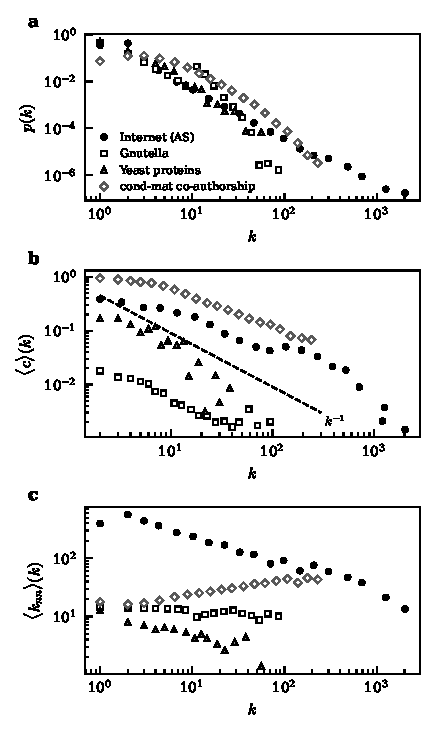
\includegraphics[width=\linewidth]{figs/fig-intro-data.pdf}
\caption{\textbf{What the data demand.} Four real networks from the Netzschleuder
repository, measured through \texttt{graph-tool}. (a) The degree distributions are
broad and hub-dominated; the Internet spans four decades of degree. Gnutella's
protocol caps its peers, so its tail is the shortest. (b) The clustering hierarchy
of Eq.~\eqref{eq:intro-hierarchy}: $\langle c\rangle(k)$ falls with degree in every
network, at roughly the advertised $k^{-1}$ (dashed guide). (c) The average
neighbor degree, where the two families part: falling for the Internet, Gnutella
and the yeast proteins --- \emph{disassortative} --- but rising for cond-mat
co-authorship, which is \emph{assortative}.}
\label{fig:intro-data}
\end{figure}

These regularities are robust, they hold across many orders of magnitude in
network size, and for years their shared origin was a mystery. Supplying that
origin, one mechanism and one class of networks at a time, is the work of this
book.

\section{Plan of the book}

The chapters proceed from mechanism to application, each built around one
concrete local rule and a family of real networks it illuminates. The reader
need not take any chapter on faith: in each, a simple local rule is stated, its
consequences are worked out (with the heavier algebra confined to boxes that can
be skipped), and the predictions are held up against real data.

\begin{itemize}
  \item \textbf{Search and connect.} A newcomer learns of existing nodes by
    exploring the network --- following references, surfing hyperlinks,
    performing a random walk --- and connects to what it finds. This is the
    natural model for searchable, directed networks such as the citation network
    and the World Wide Web, and it is where we show in detail how the simple act
    of surfing manufactures an effective ``rich get richer.''

  \item \textbf{Friends of friends.} A newcomer connects to a node and then to
    some of that node's neighbors --- you meet a person, then their friends. This
    rule for social network growth creates triangles directly, and it generates
    the assortative correlations and the cliquishness hierarchy of social
    networks.

  \item \textbf{Gene duplication.} Biological networks grow by copying: a node is
    duplicated together with its connections, after which links are gained and
    lost. Duplication is an intrinsically local move, and it explains the
    disassortative, hierarchical structure of protein interaction networks.

  \item \textbf{Activity specialization.} The schedule of a large project is a
    network of activities grown by a local refinement rule: each activity is
    either duplicated into parallel copies or split into specialized sequential
    parts. The same copying mechanism gives power-law degrees, while making the
    celebrated ``critical path'' vanish as projects grow and relocating delay
    risk in the network as a whole.

  \item \textbf{Emergence of communities.} Local rules do not only set degrees
    and correlations; they also organize nodes into communities --- tight groups
    with many links inside and few outside. We examine how this mesoscale
    structure arises from the same local dynamics, even when every node is
    otherwise identical.

  \item \textbf{Boosting shortest path multiplicity.} Finally we turn to the
    redundancy of routes through a network --- how many equally short paths join
    two nodes --- and show that local growth multiplies them, tying this
    redundancy to the very community structure of the previous chapter.
\end{itemize}

A single thread runs through all of them. In each case the apparently global
features of a network --- its scale-free degrees, its small-world distances, its
clustering hierarchy, its degree correlations, its communities, its redundant
paths --- turn out to be the collective, emergent consequence of simple rules that
no node applies with more than local knowledge. That is the sense in which the
title of this book should be read: not networks built by a designer, but networks
that grow themselves, one local decision at a time.
